\documentclass[12pt]{article}

\usepackage[margin=1.2in]{geometry}
\usepackage[parfill]{parskip}
\usepackage{graphicx}
\usepackage{float}

\begin{document}
\title{A GPS Application for the Nokia N900}
\author{Kevin Burns, Victoria Chwalowski, Matthew Via}
\date{}
\maketitle

\section{Description of Program}
This program takes input from the accelerometer and GPS on the N900 and creates
a colorized GPS trace. As the user moves, GPS data points are stored and
displayed in a widget on the right side of the screen. The color of each point is controlled by the
accelerometer. Each axis determines the value of either the red, green, or blue
component of the color. The current value of each component is displayed on
three sliders on the left side of the main window. As the phone is tilted from side to side, the current
color changes, and is displayed as the background of the main window. 

A drop-down menu at the top of the screen has four options: Settings, Open
Trace, Save Trace, and Reset Trace. In the Settings window, the user can select
which RGB components should be paired with which axis - X, Y, or Z. Open Trace
will open a file containing a previous GPS trace, display it on the screen, and
start adding data points to it. Save Trace will dump the list of the GPS data
points to a file so that it can be opened later. Reset Trace deletes the current
list of data points and clears the GPS trace display.

\section{Diagrams}
\begin{figure}[H]
  \centering
    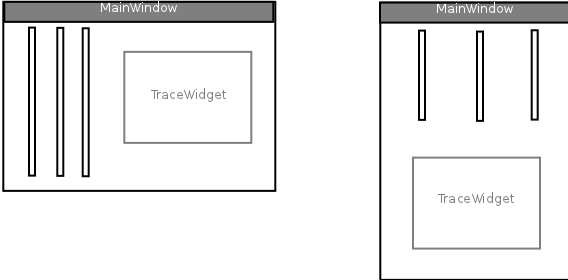
\includegraphics{mainwindow.png}
  \caption{The MainWindow, with three sliders and a TraceWidget, in both
  orientations.}
\end{figure}

\begin{figure}[H]
  \centering
    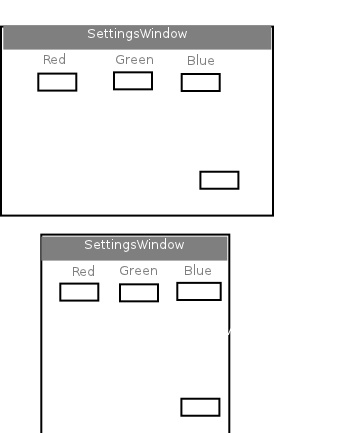
\includegraphics{settingswindow.png}
  \caption{The SettingsDialog, with three QLabels and three QComboBoxes, in both
  orientations.}
\end{figure}

\subsection{Base Classes}
\begin{description}
\item[MainWindow] \hfill \\
MainWindow, an extension of a QMainWindow, is the main application window for
the GPS app.  It contains the sliders and the TraceWidget.  It also maintains
the DataPointList of GPS data points, and is the receiver of all signals related
to the accelerometer and the GPS.
\item[SettingsDialog] \hfill \\
SettingsDialog, a subclass of QDialog, is a pop-up dialog that allows the
selection of which Axis controls what colour.  The QDialog's accept() slot is
overridden to call the main window's commitSettings (to update the settings
changed in the dialog).
\item[MapDataPoint] \hfill \\
MapDataPoint is a simple wrapper data structure to hold a GPS data point
(latitude/longitude) and the accelerometer values (X, Y, Z) when that data point
was captured.  It also contains friend functions to allow easy reading from and
writing to a QTextStream.  This makes the serialization of the data points (for
saving/reading a file) much easier.
\item[DataPointList] \hfill \\
DataPointList is a subclass of a QLinkedList typed to hold only pointers to
MapDataPoints.  It is different from a normal QLinkedList in that it knows the
bounds on all the GPS data points in the list.  It can be instantiated with a
minimum coverage (in latitude/longitude), and the append() function is
overridden so that when adding a new data point, the bounds are also updated to
include the new data.
\item[TraceWidget] \hfill \\
TraceWidget is a subclass of QWidget.  The main purpose is to provide a
dedicated widget to the trace display.  It overrides the paintEvent() function
so that upon updating, the DataPointList is iterated over and all points are
shown.  The viewport is used in such a way to make the display agnostic as to
the size of the physical window on a screen.  Whenever something is updated (new
GPS data, or a slider change) in the main window, TraceWidget's update() is
called to redraw.
\end{description}

\section{Design of QPainter graphics}
The QPainter system was used in two separate places in the GPS app.  All
QWidgets inherit from QPaintDevice, which gives them all the function paintEvent().
This function is called whenever the window needs to repaint itself -- either
from some window event (such as being unhidden), or a direct call to update() or
repaint().  

The main use of QPainter was in the TraceWidget class.  The TraceWidget
contained a pointer to the current in-use DataPointList, and has an overriden
paintEvent().  Each time paintEvent is called, the TraceWidget iterates over the
data point list and uses a QPainter instance to draw to the widget.  The only
actual drawing function that was used from QPainter was drawEllipse() to draw
points that are large enough to be easily seen on the screen.

Since the MainWindow class is also a QWidget and also is a QPaintDevice, we were
able to override its paintEvent() function as well.  This was done as a simple
way of showing the current accelerometer-based color that would be saved to the
trace.  To do this, QPainter's fillRect was used with the painter's viewport as
a bounding box.  

\section{Responsibilities}
Burns and Chwalowski created the original application, which only took
accelerometer input and displayed the current color in a QTextBox on the screen.
Via added the menu bar and settings window to this program, which allowed
changing which axis controlled which component. Chwalowski changed the layout of
the program so that objects displayed correctly when the orientation of the
phone changed.

When a QPainter had to be added, the group decided to utilize the N900's GPS to
create a colorized trace. Via created the MapDataPoint and DataPointList classes
to store GPS data, and made a TraceWidget that could display traces. Chwalowski
fixed the layout again and installed the application onto the phone.

Chwalowski created the report template in LaTeX and wrote a significant amount
of documentation, and Burns made the diagrams of
the program. Via also contributed documentation of the base classes to the
report.

\section{Problems}
One major problem was changing the layout of objects when the orientation of the
phone changed.  Simply changing our previous QTextEdit (used for displaying the
color) to the newly created TraceWidget broke most of the layout, despite the
fact that the UI settings were exactly the same.

Another issue was getting the sizing correct for the TraceWidget to display
latitude/longitude points.  Points can only be drawn in integer number spaces.
As a simple solution, we multiplied all coordinates by a large number (10000),
including the viewport dimensions.  Getting the logic for sizing the viewport to
best see the data points was not entirely intuitive, and relies more on
heuristics from trial and error than some possible designs.


\end{document}
